% xetex compatible variant that support TTF fonts according to company rules
\documentclass[ignorenonframetext, professionalfonts, hyperref={unicode}]{beamer}

\usetheme{Epam}

\usepackage{fontspec}
\setsansfont{SourceSansPro-Regular}
%\setbeamerfont{frametitle}{family=\fontspec{Oswald}}
\setbeamerfont{frametitle}{family=\fontspec{Oswald}}
\setbeamerfont{block title}{family=\fontspec{Oswald}}

%\setmainfont{Times New Roman}
\defaultfontfeatures{Mapping=tex-text}
\defaultfontfeatures{Ligatures=TeX}

%\setsansfont{Arial}
%\setromanfont{Trebuchet MS}

\usepackage{cmap}
\usepackage{graphicx}

\usepackage{textcomp}

\usepackage{beamerthemesplit}

\usepackage{ulem}

\usepackage{verbatim}
\usepackage{import}

\usepackage{listings}
\lstloadlanguages{bash}

\lstset{escapechar=`,
	captionpos=b,
	extendedchars=false,
	language=sh,
%	frame=single,
	tabsize=2, 
	columns=fullflexible, 
%	basicstyle=\scriptsize,
	keywordstyle=\color{blue}, 
	commentstyle=\itshape\color{brown},
%	identifierstyle=\ttfamily, 
	stringstyle=\mdseries\color{green}, 
	showstringspaces=false, 
	numbers=left, 
	numberstyle=\footnotesize, 
	breaklines=true, 
	inputencoding=utf8,
	keepspaces=true,
	morekeywords={u\_short, u\_char, u\_long, in\_addr}
	}

\definecolor{darkgreen}{cmyk}{0.7, 0, 1, 0.5}

\lstdefinelanguage{diff}
{
    morekeywords={+, -},
    sensitive=false,
    morecomment=[l]{//},
    morecomment=[s]{/*}{*/},
    morecomment=[l][\color{darkgreen}]{+},
    morecomment=[l][\color{red}]{-},
    morestring=[b]",
}

\author[Epam]{{\bf Epam}\\Low Level Programming Department}

%\institution[EPAM]{EPAM}
%\logo{\includegraphics[width=1cm]{logo.png}}

\graphicspath{{../../slides/cmdline/clipart/}{../../slides/bash/clipart/}}

\bibliographystyle{unsrt}
\setbeamertemplate{bibliography item}{\insertbiblabel}

\AtBeginSection[]{%
  \begin{frame}<beamer>
    \frametitle{}
    \tableofcontents[
        sectionstyle=show/shaded, hideallsubsections ]
  \end{frame}
  \addtocounter{framenumber}{-1}% If you don't want them to affect the slide number
}

% \regex for regular expressions
\newcommand{\regex}[1]{ %
\expandafter{$\ulcorner{\color{blue}\texttt{#1}}\lrcorner$} %
}



\title{Введение в GNU/Linux}

%%%%%%%%%%%%%%%%%%%%%%%%%%%%%%%%%%%%%%%%%%%%%%%%%
%%%%%%%%%% Begin Document  %%%%%%%%%%%%%%%%%%%%%%
%%%%%%%%%%%%%%%%%%%%%%%%%%%%%%%%%%%%%%%%%%%%%%%%%

\begin{document}

\begin{frame}
	\frametitle{Networking}
	\titlepage
	\vspace{-0.5cm}
	\begin{center}
	%\frontpagelogo
	\end{center}
\end{frame}


\begin{frame}
	\tableofcontents
	[hideallsubsections]
\end{frame}

%%%%%%%%%%%%%%%%%%%%%%%%%%%%%%%%%%%%%%%%%   
%%%%%%%%%% Content starts here %%%%%%%%%%
%%%%%%%%%%%%%%%%%%%%%%%%%%%%%%%%%%%%%%%%%

\section{Network basics TCP/IP}
\mode<all>{\begin{frame}{Ethernet Frame}

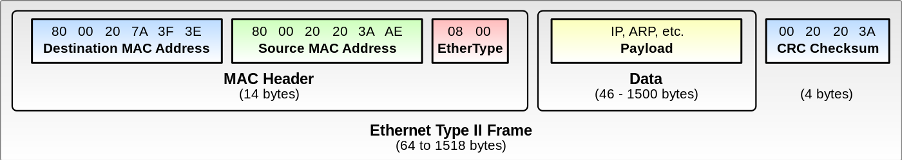
\includegraphics[width=0.95\textwidth]{../../slides/networking/net_eth_frame.png}

\end{frame}


}
\mode<all>{\begin{frame}{IP пакет}

	\center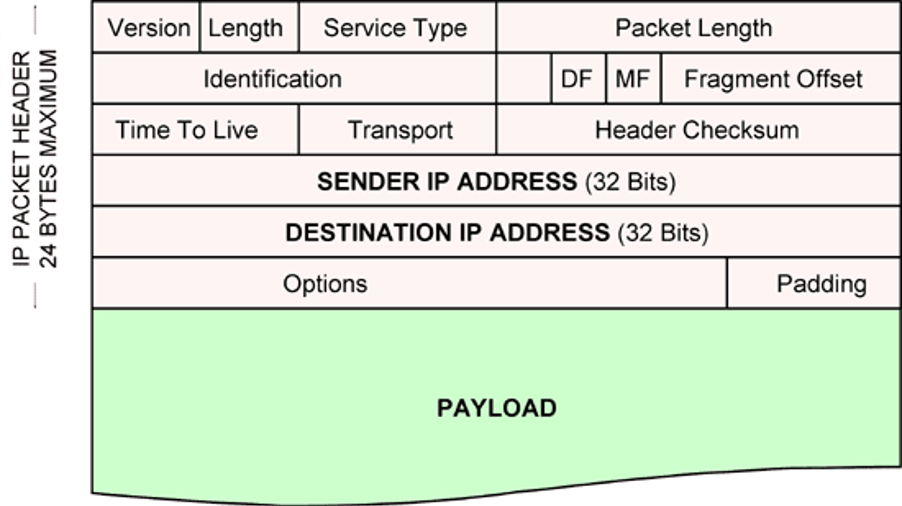
\includegraphics[width=0.9\textwidth]{../../slides/networking/net_IP_head.png}

\end{frame}


}
\mode<all>{\begin{frame}{Cегмент TCP}

	\center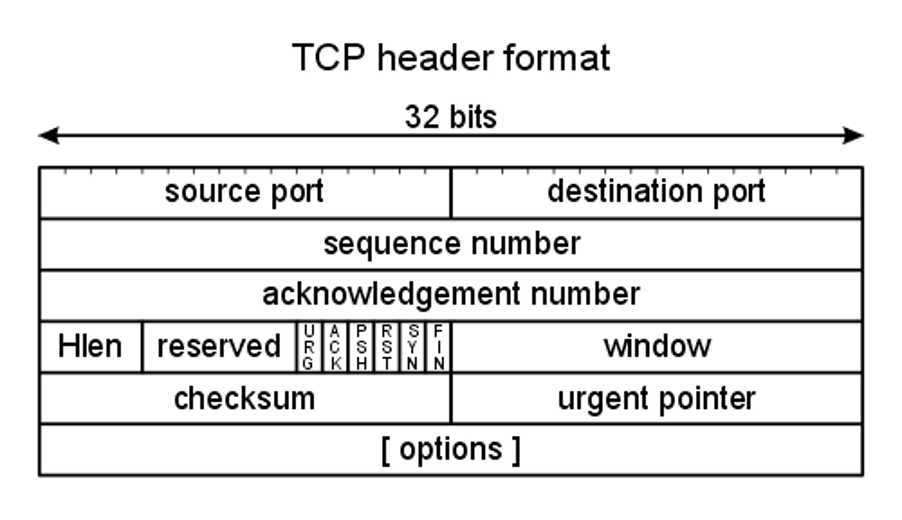
\includegraphics[width=0.9\textwidth]{../../slides/networking/net_TCP_head.png}

\end{frame}


}
\mode<all>{\begin{frame}{Инкапсуляция}

	\center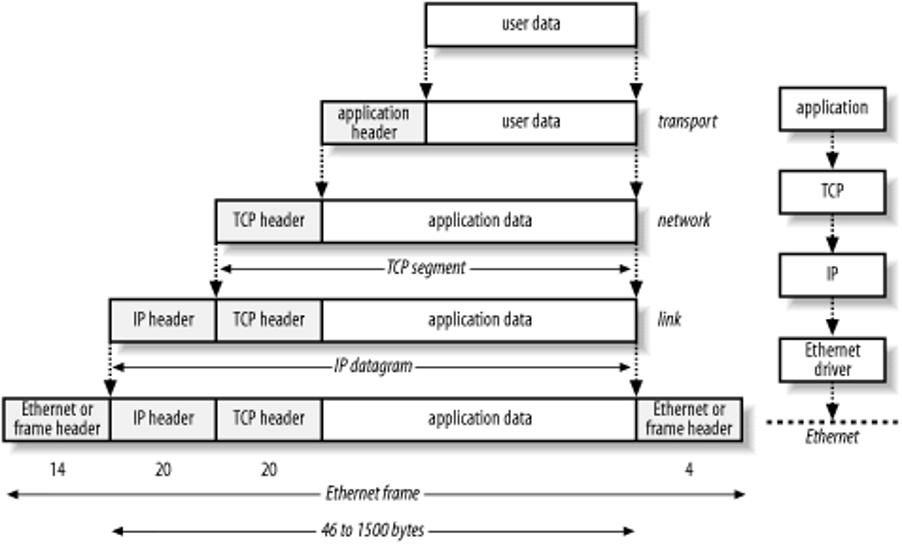
\includegraphics[width=0.9\textwidth]{../../slides/networking/net_encapsulation.png}

\end{frame}


}
\mode<all>{
\begin{frame}{Анализируем сетевой трафик}
Соберем пакеты сниффером
	\begin{itemize}
		\item tcpdump
		\item tshark 
		\item wireshark
	\end{itemize}
Из заголовков найдем MAC, IP, Ports
\end{frame}}
\mode<all>{
\begin{frame}{Выбирем диапазон IP}
Приватная сеть RFC 1918
	\begin{itemize}
		\item 127.0.0.1
		\item 10.0.0.0        -   10.255.255.255  (10/8 prefix)
		\item 172.16.0.0      -   172.31.255.255  (172.16/12 prefix)
		\item 192.168.0.0     -   192.168.255.255 (192.168/16 prefix)
	\end{itemize}
	http://jodies.de/ipcalc
\end{frame}}
\section{Configure network settings}
\mode<all>{\begin{frame}{Имена интерфейсов}
	\begin{itemize}
		\item enb0s3 - Ethernet интерфейс (аналог ethN)
		\begin{itemize}
			\item b – on-board интерфейс,
			\item 0 – номер интерфейса
			\item s3 – номер слота подключения)
		\end{itemize}
		\item wlp0s3 – Wi-Fi интерфейс.
		\item wwp0s2 - интерфейс dial up модемом, PPTP vpn, или 3G USB модемом
	\end{itemize}
\end{frame}


}
\mode<all>{\begin{frame}{Configure network interface}
Minimal settings are:
  \begin{itemize}
    \item IP address 
    \item Netmask 
	\item Gateway
    \item DNS server (optional)
  \end{itemize}
Why do you need static configuration? \\ 
Dynamic host configuration protocol (DHCP). DHCP server can be built-in:
  \begin{itemize}
	\item Server
    \item Modem 
    \item Hypervisor 
  \end{itemize}
	or run DHCP as standalone service
\end{frame}

\begin{frame}{Network configuration via commands}
\lstinputlisting[language=bash]{../../slides/networking/samples/example_network_configuration.txt}
\end{frame}

\begin{frame}[fragile]{Ubuntu network configuration files}

Configuration file: {\tt /etc/network/interfaces }

\begin{block}{Dynamic IP Address Assignment}
    \begin{lstlisting}
auto eth0
iface eth0 inet dhcp
    \end{lstlisting}
\end{block}

\begin{block}{Static IP Address Assignment}
    \begin{lstlisting}
    auto eth0
    iface eth0 inet static
    address 10.0.0.100
    netmask 255.255.255.0
    gateway 10.0.0.1
    \end{lstlisting}
\end{block}
\end{frame}

\begin{frame}{Network configuration files}
  \begin{itemize}
    \item {\tt /etc/sysconfig/network}
    \item Расположение зависит от дистрибутива:
        \begin{itemize}
            \item RH-like: {\tt /etc/sysconfig/network-scripts}\\
                {\tt /etc/sysconfig/network-scripts/ifcfg-eth0}
            \item ALTLinux: {\tt /etc/net/ifaces}
            \item Debian: {\tt /etc/network/interfaces}
            \item Gentoo: {\tt /etc/conf.d/net}
        \end{itemize}
  \end{itemize}
\end{frame}

\begin{frame}[fragile]{CentOS network configuration files}
Configuration file: {\tt /etc/sysconfig/network-scripts/ifcfg-<interface-name> }

\begin{block}{Dynamic IP Address Assignment}
    \begin{lstlisting}
DEVICE=eth0
BOOTPROTO=dhcp
ONBOOT=yes
    \end{lstlisting}
\end{block}

\begin{block}{Static IP Address Assignment}
    \begin{lstlisting}
DEVICE=eth0
BOOTPROTO=static
ONBOOT=yes
NETMASK=255.255.255.0
IPADDR=10.0.1.27
    \end{lstlisting}
\end{block}
\end{frame}

\begin{frame}[fragile]{Apply configuration settings}
    \begin{lstlisting}
    ifdown eth0
    ifup eth0
    \end{lstlisting}
    CentOS manage network configuration
    \begin{lstlisting}
    systemctl status network.service
    systemctl restart network.service
    \end{lstlisting}
    Ubuntu manage network configuration
    \begin{lstlisting}
    systemctl status networking.service
    systemctl restart networking.service
    \end{lstlisting}
\end{frame}


\begin{frame}[fragile]{Host name resolution}
\begin{block}{ {\tt /etc/resolv.conf}}
        \begin{lstlisting}
        domain it-academy.by
        search it-academy.by
        nameserver 217.23.115.244
        nameserver 192.168.37.1
        \end{lstlisting}
    \end{block}
\begin{block}{ {\tt /etc/hosts} }
        \begin{lstlisting}
        127.0.0.1 localhost
        127.0.1.1 zabbix
        \end{lstlisting}
\end{block}
\end{frame}
}
\section{Network diagnostic}
\mode<all>{\begin{frame}{Полезные утилиты}
	\begin{center}
		\begin{itemize}
			\item netstat / ss
			\item nslookup / dig
			\item ping
			\item traceroute
			\item tcpdump
			\item telnet
			\item netcat
			\item nmap
		\end{itemize}
	\end{center}

\end{frame}


%\begin{frame}{Полезные утилиты: практика}
%
%	\begin{columns}
%		\column{0.5\textwidth}
%		\begin{block}{netstat}
%
%			Узнать:
%			\begin{itemize}
%				\item список используемых сокетов
%				\item серверных сокетов
%				\item имена/pid серверов
%				\item узнать номера портов
%			\end{itemize}
%		\end{block}
%	
%		\pause
%		\column{0.5\textwidth}
%		\begin{block}{telnet/netcat}
%
%			\begin{itemize}
%				\item Чат по протоколу TCP с соседом
%				\item Чат по протоколу UDP с соседом
%				\item Передать текстовый и бинарный файлы
%			\end{itemize}
%	
%			При создании чата использовать {\tt netstat} и {\tt tcpdump}
%			для получения информации о соединении.
%		\end{block}
%	
%	\end{columns}
%\end{frame}
%
%nmap
%1. сканирование соседа
%2. сканирование выделенных портов у соседа (поиск сервера чата) 
%3. узнать список открытых портов на всех машинах в 505
%4. узнать список  работающих машин
%
%tcpdump
%0. pcap файлы/libpcap
%1. запуск монитора
%2. запуск чата
%3. монитор-фильтр-анализ
%
}
\section{Routing}
\mode<all>{\input{../../slides/networking/routing}}
\section{Firewall}
\mode<all>{\input{../../slides/networking/iptables}}

\end{document}
